\chapter{Grundlagen von Cloud Computing}
\putz

%Quellen: Reisi Folien, %Quellen: Reis Folien, https://de.wikipedia.org/wiki/Cloud_Computing#Servicemodelle

\section{Cloud Computing Definition}
\subsection{Allgemeines}
Es gibt einige verschiedene Definition des Begriffs Cloud Computing, einer sehr präzise Beschreibung wäre:

\begin{center}
   \textit{Ein Modell zur Bereitstellung von einer Reihe von Services für Unternehmen oder anderweitige Konsumenten über das Internet, wie zum Beispiel das
	Speichern von bestimmten Daten oder das Hosten einer Webseite auf einem Webserver. Die Services sind nicht nur auf Software Angebote beschränkt, es kann zum Beispiel auch Rechenleistung
	angeboten werden. Der Service läuft aus der Sicht des Konsumenten extern beim Anbieter der Services, dem sogenannten Provider.}
\end{center}

Jede Cloud hat bestimmte Eigenschaften welche den Begriff definieren, diese teilen sich in drei Hauptbereiche aus:
\begin{itemize}
	\item die zentralen, essenziellen Charakteristiken einer Cloud
	\item Servicemodelle
	\item Deployment Models oder Bereitstellungsmodelle
\end{itemize}

%Quellen: Reis Folien, https://de.wikipedia.org/wiki/Cloud_Computing

\subsection{Charakteristiken einer Cloud}
Jede Cloud hat bestimmte spezielle Charakteristiken, das NIST \textbf{(National Institute of Standard and Technology)} listet
momentan fünf essenzielle Eigenschaften die da wären:
\begin{itemize}
	\item \textbf{On-demand self-service: } Bedeutet, dass Ressourcen wie etwa Speicher und Rechenleistung der Cloud, vom Nutzer selbstständig oder automatisiert 
ohne persöhnliche Interaktion mit dem Service Provider in Anpsruch genommen werden kann
	\item \textbf{Broad network access: } Services aus der Cloud sind über das Internet und durch Standardmechanismen, mithilfe von verschiedenen Plattformen
wie einem Smartphone, einem Laptop, einem Stand-PC oder Tablet, erreichbar
	\item \textbf{Resource pooling: } Die in generell in einer Cloud zu Verfügung stehenden Ressourcen wie zum Beispiel Speicher und Rechenleistung sind für alle Kunden gebündelt von einem Pool aus verfügbar und werden geteilt, dabei ist der physische Standort der Server für den Klienten in der Regel unbekannt.
	\item \textbf{Rapid elasticity: } Die durch den Kunden in Anspruch genommenen Ressourcen können aus dessen Sicht, schnell ins beinahe unendliche skaliert werden, die Lastenänderung
kann ebenfalls automatisiert angepasst werden, sodass keine menschliche Interaktion notwendig ist.
	\item \textbf{Measured Service: } Die Ressourcennutzung der Kunden kann durch den Anbieter gemessen, überwacht und analysiert werden, zum Zwecke von Abrechnungen, einer effektiver
Nutzung der in Anspruch genommenen Ressourcen oder für eine vorausschauende Gesamtplanung.
\end{itemize}

%Quellen: Reis Folien, https://de.wikipedia.org/wiki/Cloud_Computing#Servicemodelle,
%https://azure.microsoft.com/de-de/overview/what-is-cloud-computing/#cloud-computing-models

\subsection{Servicemodelle}
NIST listet drei grundsätzliche Standard-Modelle, in welcher Form Cloud Computing Dienste angeboten werden können, diese werden oft als Schichten untereinander vereinfacht dargestellt:
\begin{itemize}
	\item Infrastructure as a Service (IaaS)
	\item Platform as a Service (PaaS)
	\item Software as a Service (Saas)
\end{itemize}


Zusätzlich zu den oben genannten standardisierten Modellen, existieren noch einige weitere Modelle auf dem Markt. Prinzipiell
kann man heutzutage fast jeden nur denkbaren Service über eine Cloud beziehen, mit der Zeit haben sich dafür spezielle Bezeichnungen gebildet. Diese Fachbegriffe können zusammengefasst werden:
\begin{itemize}
	\item Function as a Service (FaaS) oder Serverless computing
	\item Everything as a Service (XaaS)

\end{itemize}

%Quellen: Reis Folien, https://de.wikipedia.org/wiki/Cloud_Computing#Servicemodelle,
%https://azure.microsoft.com/de-de/overview/what-is-cloud-computing/#cloud-computing-models,
%https://de.wikipedia.org/wiki/Everything_as_a_Service#Infrastructure_as_a_Service_(IaaS),

\subsubsection{Infrastructure as  a Service (IaaS)}
Bei IaaS nimmt der Kunde IT-Infrastruktur wie Server, Speicher und Virtuelle Computer von einem Cloudanbieter in Anspruch. In diesem Fall gestaltet der Kunde seine eigene Infrastruktur selbst innerhalb einer Cloud und kümmert sich um die Installation von Software und den laufenden Betrieb derer selbst. Der Anbieter ist lediglich für die genutzten physischen Hardware Elemente verantwortlich und wartet diese, alles andere fällt in den Zuständigkeitsbereich des Kunden. Kurz zusammengefasst ist IaaS Bereitstellung von Infrastruktur über das Internet, welche vom Nutzer bedingt kontrolliert wird. \newline
Infrastructure as a Service kann auch als Everything as a Service bezeichnet werden, da in diesem Geschäftsmodell alles vom Kunden selbst verwaltet wird. Einige Charakteristiken von IaaS:
\begin{itemize}
	\item Nur einmalig genutzte Anwendungen werden einmal bezahlt und wieder freigegeben
	\item Im Falle eines explosionsartigen Wachstums und ein erreichen der Belastungsspitzen kann abgefangen werden, da die Services in jede Richtung skalierbar sind. So können innerhalb von Minuten zum Beispiel viel Speicher erweitert werden oder auch im Gegenteil nicht genutzte Kapazitäten frei gegeben werden, welche dann nicht mehr bezahlt werden müssen.
\end{itemize}

Ein Beispiel dafür wäre das Mieten eines VPS-Servers (Virtual Private Server) um eine Webapp wie EMS darauf aufzusetzen.
Als Kunde mietet man eine gewisse Größe an Hauptspeicher (RAM) und Nebenspeicher (SSD), eine Anzahl an CPU-Kernen, wie groß die Bandbreite seien soll und noch viele andere Optionen, welche bei jedem Cloudanbieter variieren. Auf diesem VPS-Server kann man nun sein Front- und Backend aufsetzen und hat über alles selbst die Kontrolle. Klassische Anbieter welche IaaS anbieten wären Amazon mit Amazon Web Services (AWS) mit dem möglicherweise populärsten Service EC2.

%Quellen: Reis Folien, https://de.wikipedia.org/wiki/Cloud_Computing#Servicemodelle,
%https://azure.microsoft.com/de-de/overview/what-is-cloud-computing/#cloud-computing-models,
%https://de.wikipedia.org/wiki/Platform_as_a_Service

\subsubsection{Platform as a Service (PaaS)}
PaaS stellt dem Kunden eine Programmier- und Laufzeitumgebung zur Verfügung. Hier stellt der Cloudanbieter eine Softwareumgebung fertig aufgesetzt für den Nutzer zur Verfügung, damit dieser eigene Softwareanwendungen darauf entwickeln kann. Die Daten- und Rechenkapazitäten der Umgebungen sind dabei flexibel und können dynamisch hin Hinsicht auf Daten- und Rechenkapazität angepasst werden.\newline
\newline
Diese Form des Cloudservices würde sich vor allem an Unternehmen richten, welche eine große Anzahl an Mitarbeiter beschäftigt und an vielen Applikationen gleichzeitig arbeitet und diese schnell entwickeln muss, jedoch nicht genügend Kapital hat, um jeden Arbeitsplatz mit einer Rechenmaschine mit entsprechend benötigter Leistung auszurüsten. Stattdessen könnte solch eine Firma auf PaaS zurückgreifen und für einen geringen Betrag, monatlich diese Umgebungen in einer Cloud mieten und spart sich so viel Kapital und bleibt bei den benötigten Rechenleistungen flexibel, da die Umgebungen eben flexibel auf die benötigten Performanceansprüche skaliert werden kann. Dies wäre bei eingekaufter Hardware in einem Büro nicht so leicht, was dieses Servicemodell den Kunden auch schnell und einfach auf neue Technologien und Anforderungen reagieren lässt.

%Quellen: Reis Folien, https://de.wikipedia.org/wiki/Cloud_Computing#Servicemodelle,
%https://azure.microsoft.com/de-de/overview/what-is-cloud-computing/#cloud-computing-models,
%https://de.wikipedia.org/wiki/Software_as_a_Service

\subsubsection{Software as a Service (SaaS)}
Manchmal auf als Software on Demand beschrieben, was "`Software nach Bedarf"' übersetzt bedeutet. Hier bietet der Cloudanbieter spezielle Software zur Nutzung an. Der Kunde kann dann diese Software- und Anwendungsprogramme nach belieben benutzen. Die Applikationen werden über das Internet dem Nutzer zur Verfügung gestellt, und dieser kann mittels einer API darauf zugreifen, was meistens über einen Browser oder eine App geschieht. Die Infrastruktur hinter den Anwendungen verwaltet der Anbieter selbst und auch die Angebotene Software könnte nur bis zu einem gewissen Teil vom Kunden konfiguriert werden. Also sämtliche Instandhaltungsarbeiten obliegen dem Cloudanbieter, der Nutzer benutzt lediglich die angebotene Software und kann sich bei Problemen nur an den Support wenden.\newline
\newline
Ein Beispiel für so einen Service wären die meisten Google Services wie Gmail, Docs, Drive und Photos. Noch weitere Prominente Beispiele für Software as a Service sind Github, Office 365 und Dropbox.

%Quellen: Reis Folien, https://de.wikipedia.org/wiki/Cloud_Computing#Servicemodelle,
%https://azure.microsoft.com/de-de/overview/what-is-cloud-computing/#cloud-computing-models,
%https://de.wikipedia.org/wiki/Function_as_a_Service

\subsubsection{Function as a Service (FaaS)}
Prinzipiell ist FaaS von den Angeboten und Leistungen ähnlich wie das vorhin beschriebene Paas-Modell. Es stellt eine Laufzeitumgebung zur Verfügung, worauf Softwareanwendungen erstellt werden könne. Der maßgebende Unterschied zwischen Function und Platform as a Service ist, dass bei PaaS die Skalierung mittels hinzufügen von weiteren Serverprozessen zu den bereits in Anspruch genommenen stattfindet. Dies bewirkt natürlich normalerweise eine Kostenerhöhung auf Seiten des Benutzers, welche direkt Abgebucht oder in Rechnung gestellt wird. Die Skalierung ist dem Benutzer hier dadurch aber auch sehr übersichtlich und man kann die Aus- und Belastung seiner Entwicklerumgebung leicht nachvollziehen.\newline
Ganz anders im Gegensatz dazu geschieht die Skalierung bei FaaS. Bei diesem Service läuft keine extra Serverinstanz im Hintergrund. Bei FaaS muss der Benutzer die \textbf{Function exceution time} bezahlen. Die Zeit zwischen den Ausführungen von Code wird hierbei nicht in Rechnung gestellt, also lediglich, wenn ein Code zum Beispiel Übersetzt wird oder ein Programm ausgeführt und getestet wird. Somit muss der Benutzer auch nicht mehr an die Skalierung denken, da seine Entwicklerumgebung quasi kostenlos zu Verfügung steht und er nur die Ausführung der Software nach deren Zeitaufwand bezahlen muss. Dies sorgt für geringere Kosten auf Seiten des Kunden, bei gleichzeitig höhere Skalierbarkeit, da diese nicht mehr beachtet werden muss. Einen Nachteil gibt es jedoch und zwar kann die Latenz bei diesem Server höher als bei einer Lösung mit PaaS sein. Dies ist jedoch von vielen Faktoren und nicht zuletzt auch von der Komplexität des kodierten Programmes abhängig.

Dieser Service verfolgt den Ansatz des sogenannten \textbf{"`serverless computing"'}. Hierbei übernimmt der Cloud-Anbieter die komplette Ressourcenzuweisung, zum Beispiel benötigter Speicher und benötigte Prozessorkernanzahl, für den Kunden. Bei serverless computing wird keine Ressource im volatilen Speicher gehalten. Dies bedeutet, Berechnungen werden in bestimmten Abständen durch bestimmte Events von Seiten des Kunden aus, ausgelöst und die Ergebnisse werden dann in einen persistenten Speicher geschrieben. Wenn eine Anwendung gerade nicht vom Kunden benutzt wird, wird dies auch nicht in Rechnung gestellt wie es bei herkömmlichen Services der Fall ist. Es gibt keinen fixierten Betrag der monatlich oder Quartals mäßig abgebucht wird, sondern nur produktiv genutzte Zeit in der Anwendung wird berechnet.

Das erste offizielle, kommerzielle Angebot eines solchen Services gab es 2006. Seitdem haben viele große Cloud-Anbieter wie zum Beispiel Amazon mit AWS Lambda, Google und Microsoft mit Azure, solche \textbf{pay as you go} Services zu Verfügung gestellt.

% Quellen: https://www.quora.com/What-are-the-Iaas-Paas-and-SaaS-services-in-Amazon-webservices?share=1
%https://de.wikipedia.org/wiki/Everything_as_a_Service#Weitere_Ans%C3%A4tze_2
%https://web.archive.org/web/20110728093045/http://www.thecloudcomputing.org/2009/1/panels.html#Panel2

\subsubsection{Everything as a Service (XaaS)}
XaaS oder auch EaaS, stellt prinzipiell alles zu Verfügung. Also SaaS, Paas sowie auch Iaas. Einige Anbieter spezialisieren sich auf ein bestimmtes Service Modell, manche bieten jedoch prinzipiell alle Services unter der Bezeichnung XaaS an und spalten diese Services in die spezifischere Modelle, wie zum Beispiel SaaS, auf. Dies sorgt vor allem bei Neukunden manchmal für Verwirrung. AWS (Amazon Webservices) ist so ein Service, er bietet prinzipiell jedes Modell unter XaaS an, jedoch sind hunderte weitere Services einzeln spezifiziert Verfügbar. AWS heißt lediglich das Cloud Computing System, ein tatsächlicher Service heißt zum Beispiel AWS EC2, dieser Service ist als IaaS zu spezifizieren. Hierbei kann man einen virtuellen Server mit einem bestimmten Betriebssystem, virtuelle Kernanzahl und Hauptspeicher mieten. Dieser Service kostet stündlich, egal ob er benutzt wird oder nicht. Ein weitere IaaS Service in AWS ist S3, hier kann man Speicher mieten.\newline
AWS bietet stand April 2021 über 200 verschiedenen Services in allen Servicemodellen Iaas, Paas und SaaS.
\newline
Weitere noch spezifischere Servicemodelle wie zum Beispiel High Performance Computing as a Service (HPCaaS), Data Intensive Computing as a Service (DICaaS) oder Humans as a Service (HuaaS). Können unter XaaS übergeordnet zusammengefasst werden. Für HuaaS als Beispiel gibt es den AWS Service Amazon Mechanical Turk, dieser Dienst befindet sich jedoch noch in einer Beta-Phase, hierbei wird menschliche Intelligenz wie ein Webservice genutzt.

%Quellen:
%Reis Folien
%https://de.wikipedia.org/wiki/Cloud_Computing#Organisatorische_Arten_von_Clouds
\subsection{Liefermodelle}
Im Kapitel Servicemodelle (Sektion 1.1.3) wurde die verschiedenen Modelle, welche eine Cloud anbieten kann und wie viele gleiche Hardwareeinheiten, beginnend mit der Aufteilung derer Infrastruktur bis zur Verfügungstellung einzelner Endanwendungen, für den Endkunden benutzbar gemacht wird.\newline
Im Englischen werden sie \textbf{Deployment Models} genannt, die im deutsch genannten Liefermodelle beschreiben nun, wie genau die Services unter Berücksichtigung ihrer Aufteilung in bereits genannte Servicemodelle, einem Benutzer zu Verfügung gestellt werden:
\begin{itemize}
	\item Private cloud
	\item Public cloud
	\item Hybrid cloud
	\item Community cloud
\end{itemize}

\begin{center}
\begin{figure}[h]
    \centering
    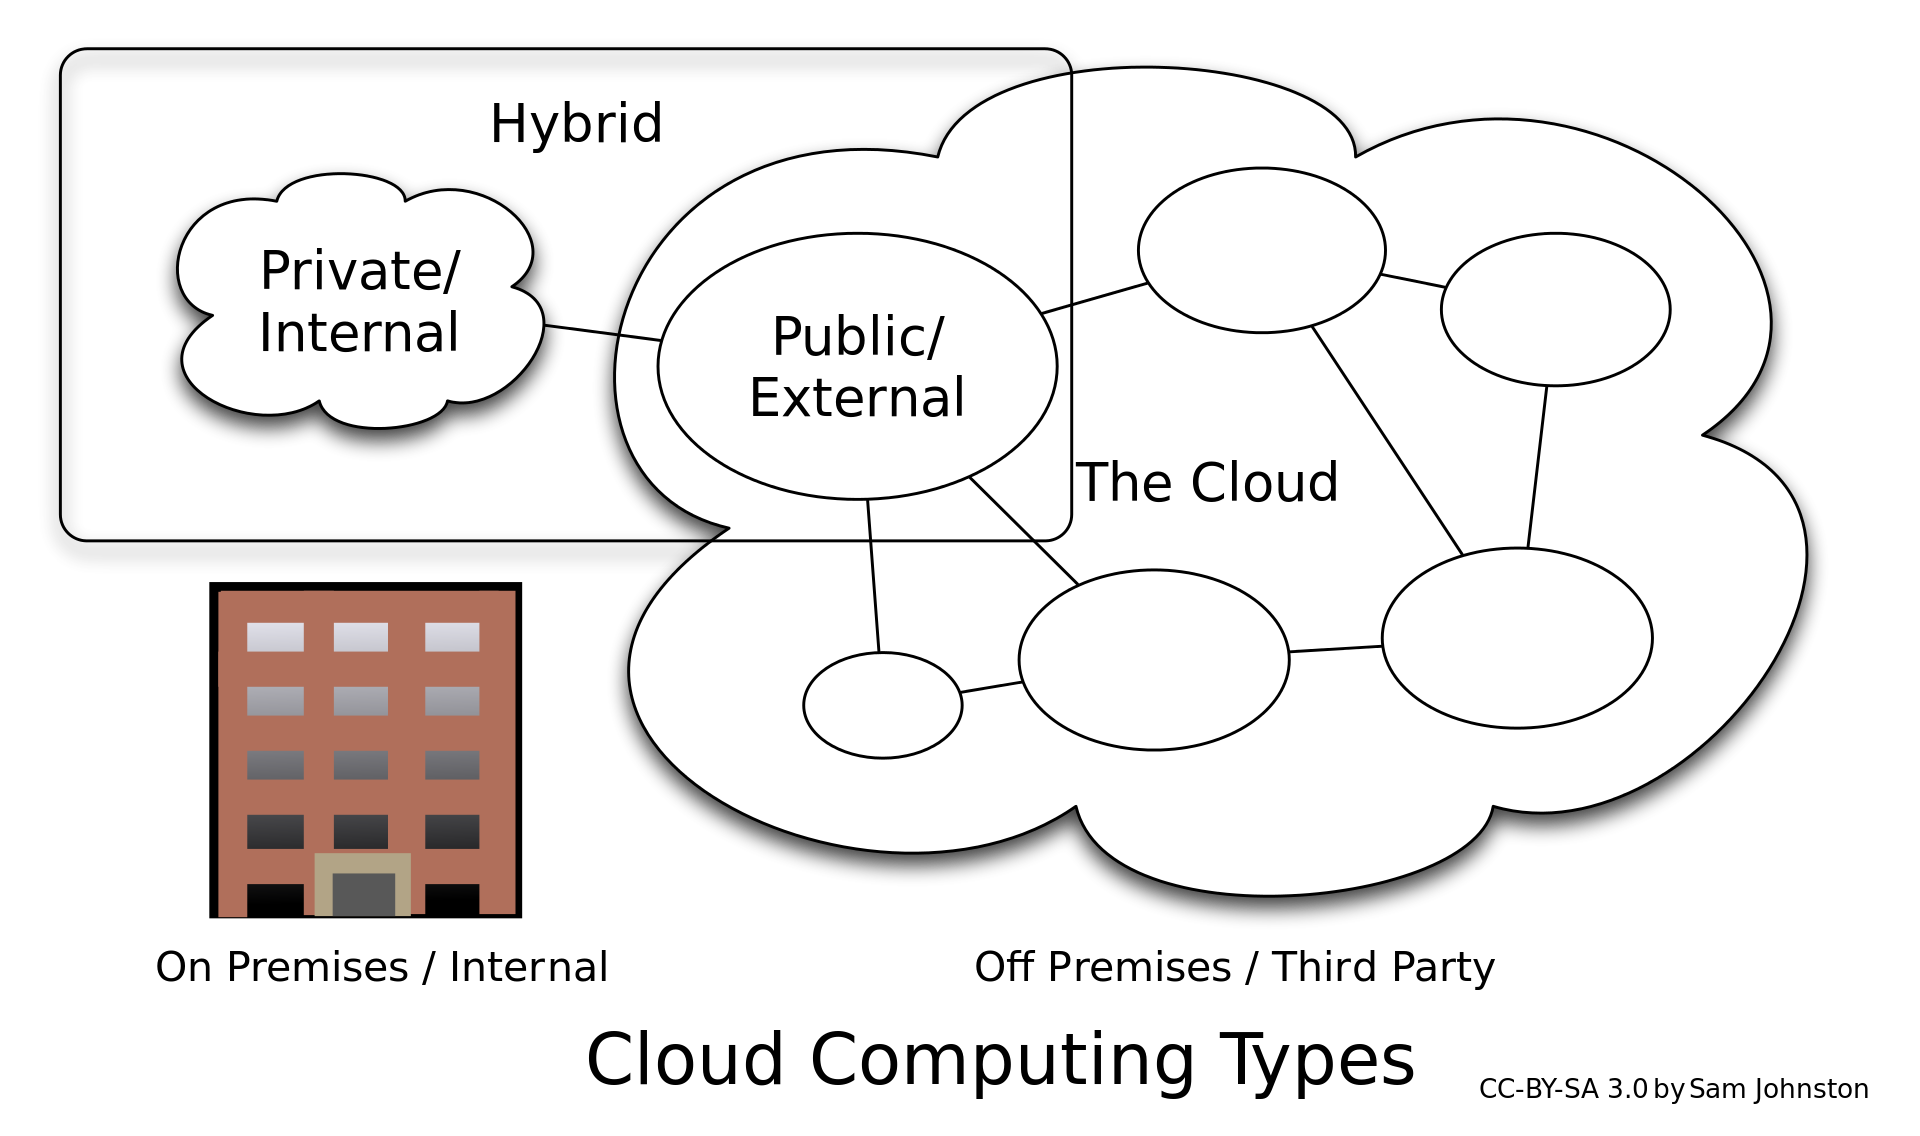
\includegraphics[width=\textwidth]{Cloud_computing_types.png}
    \caption{Liefermodelle von Cloud Computing}
\end{figure}
\end{center}

%Quellen:
%Reis Folien
%https://de.wikipedia.org/wiki/Cloud_Computing#Organisatorische_Arten_von_Clouds
%https://azure.microsoft.com/en-us/overview/what-is-a-private-cloud/
\subsubsection{Private cloud}
Private Clouds werden nur von einem einzelnen Unternehmen, einer Organisation oder einem Kunden betrieben oder stehen nur diesen und einem vertrauenswürdigen Dritten zu Verfügung. Diese Cloud-Umgebung wird entweder intern von zum Beispiel in einem firmeneigenen Rechenzentrum gehostet und verwaltet, oder aber der vertrauenswürdige Dritte übernimmt das Hosting. In letzterem Fall liegt das Rechenzentrum extern bei dem Dritten. Nicht zu verwechseln mit einem normalen IT-Betrieb, wie er in fast jedem kleinen bis mittleren Unternehmen betrieben wird. Die Bezeichnung \textbf{Private cloud} ist erst dann zutreffend, wenn alle fünf Charakteristika einer Cloud erfüllt werden (siehe Kapitel 1.1.2).
Bei einer privaten Cloud gibt es verschiedene Evolutionsstufen, welche die Wichtigkeit beziehungsweise die Verbreitung und den Nutzungsgrad innerhalb der Organisation beschreibt:
\begin{itemize}
	\item Exploratory cloud: Hier wird die Private Cloud hauptsächlich als Testumgebung parallel zum Produktivbetrieb genutzt. Oft wird sie auch, falls man sich Know-how im Gebiet des Cloud Computing anschaffen will, für Studien um Potential und Nachteilen einer internen Cloud herauszufinden, benutzt.
	\item Department cloud: Eine Cloud, die vor allem produktiv und abteilungsintern genutzt wird.
	\item Enterprise cloud: Diese Form der privaten Cloud wird im gesamten Unternehmen benutzt und ist fest im Produktivbetrieb integriert.
\end{itemize}

Microsoft bietet mit Azure einen Service an, nämlich \textbf{Azure Express Route}, welcher vor allem auf Ansprüche einer Private cloud angepasst ist.
Anwendungsfälle für eine Private cloud gibt es vor allem in Unternehmen welche Daten speichert oder verarbeitet welche im Rahmen der DSGVO unter den Begriff \textbf{sensible Daten} fällt.

%Quellen:
%Reis Folien
%https://azure.microsoft.com/en-us/overview/what-are-private-public-hybrid-clouds/
\subsubsection{Public cloud}
Eine Public Cloud für die breite Öffentlichkeit und Einzelpersonen einen Zugang zu ihren Services über das Internet. Die Kunden von Anbieter, welche eine Public Cloud betreiben, können somit jeder mit einem Internetzugang sein. Eine öffentliche Cloud kann mit drei weitere Formen genauer aufteilen:
\begin{itemize}
	\item Exclusive Cloud: Der Benutzer/Kunde und der Hoster der Cloud kennen sich persönlich durch zum Beispiel Schriftverkehr (E-Mail). Normalerweise besteht zwischen den Parteien ein individueller bilateraler Vertrag
	\item Open Cloud: In der Regel kennen sich der Benutzer/Kunde und Cloudanbieter nicht. In sogenannten \textbf{"`Service Level Agreements"'}, oder kurz SSL, werden die Leistungen und die Vergütung jeder genauestens beschrieben. Hier laufen Vertragsabschluss und Nutzung voll- oder teilautomatisiert ab, da die Anzahl der Nutzer bei dieser Form der öffentlichen Cloud viel höher als bei allen anderen ist.
	\item Virtual Private Cloud: Ein abgetrennter Bereich in einer öffentlichen Cloud, der für einen bestimmten einzelnen Kunden reserviert wird. Zusätzlich werden durch besondere Sicherheitsmaßnahmen entsprechende Vorkehrungen, für die Integrität des exklusiven Bereichs sorgen, getroffen. Ein Beispiel wäre bei Inanspruchnahme eines IaaS, die physische Trennung der gemieteten Hardware von der restlichen oder bei anderen Services ein spezieller Zugang über einen VPN.
\end{itemize}

Die bekanntesten öffentlichen Clouds sind Amazon Web Services, Google App Engine, Windows Azure und auch Salesforce.

%Quellen:
%Reis Folien
%https://de.wikipedia.org/wiki/Cloud_Computing#Organisatorische_Arten_von_Clouds
%https://en.wikipedia.org/wiki/Cloud_computing#Serverless_computing
\subsubsection{Hybrid cloud}
Das Konzept einer Hybriden Cloud besteht aus einer Mischung aus privater, öffentlicher und community cloud. Ein Beispiel für die Anwendung einer solchen Form wäre zum Beispiel, ein Unternehmen gat eine private Enterprise cloud, und nutzt aber zusätzlich als Backup falls es zum Beispiel die Belastungsspitze des System erreicht wird, eine öffentliche oder community Cloud.

%Quellen:
%Reis Folien
%https://de.wikipedia.org/wiki/Cloud_Computing#Organisatorische_Arten_von_Clouds
%https://en.wikipedia.org/wiki/Cloud_computing#Serverless_computing
\subsubsection{Community cloud}
Eine community Cloud ist ein Zusammenschluss von einigen unter sich bekannter Nutzer. Diese "`verschmolzene"' neue Cloud aus zum Beispiel einiger privaten Clouds welche einen sehr ähnlichen oder gleichen Zweck hatten, kann intern in deren Gebäuden gehostet werden, oder extern von einem Dritten betrieben werden. Die kosten dafür wird unter den ursprünglichen Teilnehmern aufgeteilt.
Ein Anbieter hierfür wäre zum Beispiel Googele Gov Cloud.


\subsection{Cloud Computing bei EMS und Wirtschaftlichkeit}

\textbf{WARTEN AUF BENNI STATISTIKEN}

\subsection{EMS und Deployment mit AWS}
Das Backend der fertigen Anwendung besteht aus den Technologien Node.Js und Express. Dieses verbindet sich mit einer externen MongoDB Datenbank in der Atlassian Cloud (siehe Kapitel 5.1.4). Grundsätzlich war geplant, dieses in der AWS Cloud unter Amazon Lightsail oder dem EC2 Service zu hosten. Stand jetzt, wird der AWS EC2 Service verwendet. Für diese Entscheidung gab es mehrere Gründe.


\newpage
 